\documentclass[11pt]{article}

\usepackage{hyperref}
\usepackage{xcolor}
\usepackage{calc}
\usepackage{graphicx}
\usepackage{tikz}
\usepackage{fontspec}
\usepackage{fontawesome5}
\usepackage{titlesec}
\usepackage{enumitem}

\hypersetup{
    hidelinks,
    unicode=true,
    pdftitle={南京信息工程大学中文简历模板（虚构示例）},
    pdfauthor={NUIST-CV 模板示例},
    pdfsubject={LaTeX 中文简历模板},
    pdfkeywords={NUIST, CV, LaTeX, 简历模板}
}

%%%%%%%%%%%%%%%%%%%%
% 页面与排版设置
%%%%%%%%%%%%%%%%%%%%

\setlength{\parindent}{0pt}
\pagenumbering{gobble}
\setlist[itemize]{
    nosep,
    before={\vspace*{-\parskip}},
    leftmargin=*
}
\renewcommand{\arraystretch}{1.2}
\linespread{1.25}

\titleformat{\section}
  {\LARGE\bfseries\raggedright}
  {}{0em}
  {}
  [{\color{secondary_color}\titlerule}]
\titlespacing*{\section}{0cm}{*1.15}{*1.05}

\usepackage[
    a4paper,
    left=1.2cm,
    right=1.2cm,
    top=1.5cm,
    bottom=1cm,
    nohead
]{geometry}

\setmainfont[
    Path=fonts/,
    Extension=.otf,
    BoldFont=*-Bold,
]{NotoSerifSC}

\definecolor{primary_color}{RGB}{18, 62, 170}
\definecolor{secondary_color}{RGB}{132, 166, 220}
\definecolor{note_color}{RGB}{95, 99, 104}

\newlength{\iconwidth}
\setlength{\iconwidth}{1.5em}

% 以下联系方式均为占位信息，example.com 是保留示例域名。
\newcommand{\contact}{
    \footnotesize
    \textcolor{white}{
        \faEnvelope \quad \href{mailto:mamba@example.com}{mamba@example.com}
        \hspace{3.5em}
        \faPhone \quad +00 824 248 0824
        \hspace{3.5em}
        \faGithub \quad \href{https://github.com/your-username}{github.com/your-username}
    }
}

\begin{document}

    % 页眉：南信大标识与示例专业名
    \begin{tikzpicture}[remember picture, overlay]
        \node[anchor=north, inner sep=0pt](header) at (current page.north){
            
\includegraphics[width=\paperwidth]{images/header-nuist-blue.png}
        };
        \node[anchor=west](school_logo) at (header.west){
            \hspace{0.5cm}
            
\includegraphics[width=0.30\textwidth]{images/nuist-white.png}
        };
        \node[anchor=east](school_name) at(header.east){
            \textcolor{white}{\textbf{数学与应用数学（凌晨四点实验班）}}
            \hspace{0.5cm}
        };
    \end{tikzpicture}
    \vspace{-3.5em}

    % 页脚：虚构联系方式
    \begin{tikzpicture}[remember picture, overlay]
        \node[anchor=south, inner sep=0pt](footer) at (current page.south){
            
\includegraphics[width=\paperwidth]{images/footer-nuist-blue.png}
        };
        \node[anchor=center] at(footer.center){\contact};
    \end{tikzpicture}

    \begin{minipage}[t]{0.78\textwidth}
        \begin{minipage}[t]{\textwidth}
        \section[个人信息]{\makebox[\iconwidth][c]{\color{primary_color}{\faAddressCard}}\quad 个人信息}
        \begin{minipage}[t]{0.5\textwidth}
            \textbf{姓\qquad 名}：科比·布莱恩特

            \vspace{0.15em}
            \textbf{出生年月}：1978.08
        \end{minipage}
        \begin{minipage}[t]{0.42\textwidth}
            \textbf{代\qquad 号}：黑曼巴

            \vspace{0.15em}
            \textbf{求职意向}：关键球负责人
        \end{minipage}
        \vspace{0.35em}
        \end{minipage}

        \begin{minipage}[t]{\textwidth}
        \section[教育背景]{\makebox[\iconwidth][c]{\color{primary_color}{\faGraduationCap}}\quad 教育背景}

        {\large \textbf{南京信息工程大学（平行宇宙）}} \hfill 1996.09--2016.04
        \begin{itemize}
            \item \textbf{专业方向}：数学与应用数学（凌晨四点实验班）
            \item \textbf{综合绩点}：\textbf{24 / 8.0，班级排名：1 / 60}
            \item \textbf{核心课程}：后仰跳投(100)、关键球(99)、录像分析(98)、晨练(100)
        \end{itemize}
        \vspace{0.35em}
        \end{minipage}
    \end{minipage}
    \hfill
    \begin{minipage}[t]{0.2\textwidth}
        \vspace{0.5em}
        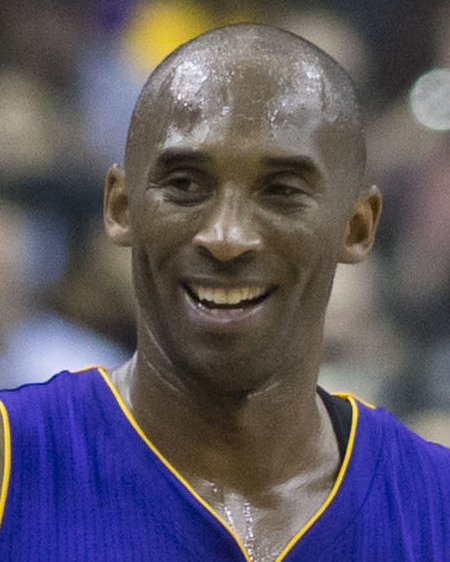
\includegraphics[width=\linewidth]{images/kobe-bryant-portrait.jpg}
    \end{minipage}

    \begin{minipage}[t]{\textwidth}
    \section[科研经历]{\makebox[\iconwidth][c]{\color{primary_color}{\faAtom}}\quad 科研经历}

    \textbf{研究项目《凌晨四点的投篮命中率：一种自监督训练范式》}
    \hfill \textbf{独立一作}
    \begin{itemize}
        \item \textbf{问题定义}：将“再练五百个”形式化为带体能约束的动态停机条件。
        \item \textbf{方法设计}：融合脚步特征、出手轨迹与防守者表情，构建端到端后仰跳投管线。
        \item \textbf{实验结果}：在 8 号与 24 号两组初始化上均稳定收敛，关键球置信度显著提升。
        \item \textbf{复现说明}：数据、代码与结论均为模板占位内容，正式使用时请替换为真实经历。
    \end{itemize}
    \vspace{0.35em}
    \end{minipage}

    \begin{minipage}[t]{\textwidth}
    \section[竞赛经历]{\makebox[\iconwidth][c]{\color{primary_color}{\faTrophy}}\quad 竞赛经历}
    \textbf{NBA 总冠军（示例履历条目）} \hfill 2000--2002、2009--2010 \quad \textbf{五次}\\[0.2em]
    \textbf{NBA 全明星（示例履历条目）} \hfill 1998、2000--2016 \quad \textbf{十八次}\\[0.2em]
    \textbf{单场投篮优化挑战} \hfill 2006.01 \quad \textbf{81 个有效样本}\\[0.2em]
    \textbf{动画短片项目《亲爱的篮球》} \hfill 2018.03 \quad \textbf{奥斯卡获奖}
    \vspace{0.35em}
    \end{minipage}

    \begin{minipage}[t]{\textwidth}
    \section[所获荣誉]{\makebox[\iconwidth][c]{\color{primary_color}{\faMedal}}\quad 所获荣誉}
    \begin{minipage}[t]{0.48\textwidth}
        \textbf{8 号球衣退役} \hfill 2017.12\\[0.2em]
        \textbf{凌晨四点全勤奖} \hfill 长期有效
    \end{minipage}
    \hfill
    \begin{minipage}[t]{0.48\textwidth}
        \textbf{24 号球衣退役} \hfill 2017.12\\[0.2em]
        \textbf{后仰跳投终身成就奖} \hfill 模板限定
    \end{minipage}
    \vspace{0.9em}
    \end{minipage}

    \begin{minipage}[t]{\textwidth}
    \section[技能特长]{\makebox[\iconwidth][c]{\color{primary_color}{\faWrench}}\quad 技能特长}
    \begin{itemize}
        \setlength{\itemsep}{0.25em}
        \item 熟练掌握后仰跳投、低位脚步与比赛录像分析，能够独立完成从训练到复盘的闭环。
        \item 能在高压环境下进行关键球决策，并为每一次打铁补充可复现的误差分析。
        \item 了解 Python、C++ 与 \LaTeX，擅长把训练计划写成永远跑不完的循环。
    \end{itemize}
    \vspace{0.25em}
    \end{minipage}

    \begin{minipage}[t]{\textwidth}
    \section[自我评价]{\makebox[\iconwidth][c]{\color{primary_color}{\faStar}}\quad 自我评价}
    \begin{itemize}
        \item 目标明确：闹钟响之前已经到场；对空位、错别字和多余空格保持同等敏感。
        \item 本页为开源简历模板的虚构戏仿示例，不代表人物本人、其相关方或任何机构。
    \end{itemize}
    \end{minipage}

\end{document}
